\section{Budowa aplikacji}
\begin{figure}[H]
	\centering
	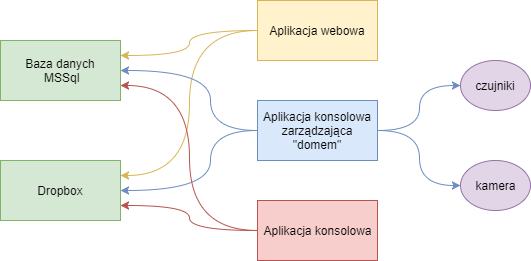
\includegraphics[scale=0.8]{schemat_systemu.png}
	\caption{Budowa systemu zarządzania domem}
	\label{fig:schemat_systemu}
\end{figure}
Aplikację powstałą na potrzeby tej pracy można podzielić na 3 moduły, które zostały przedstawione na rysunku \ref{fig:schemat_systemu}, a składają się na nie :
\begin{itemize}
\item Aplikacja webowa- interfejs pozwalający na zlecanie nowych zadań aplikacji konsolowej, odczyt wyników przesłanych przez obie aplikacje konsolowe,
\item Aplikacja konsolowa- przetwarza zadania detekcji oraz rozpoznawania twarzy zlecone za pomocą aplikacji webowej,
\item Aplikacja konsolowa zarządzająca domem- przekazuje cyklicznie odczytywane dane z czujników %\textcolor{red}{oraz wykryte ruchy do bazy danych}, w celu dalszej obróbki przez pozostałe moduły%.
\end{itemize}
We wczesnej fazie projektu istniała jedna aplikacja konsolowa, ale ze względu na skomplikowaność programu przetwarzającego zadania, została ona rozdzielona na aplikację, która musi być uruchamiana na Raspberry Pi (program zarządzający domem) oraz drugą, którą można uruchomić w dowolnym innym środowisku.s
Na usługi pomocnicze wykorzystane w projekcie składają się
\begin{itemize}
\item baza danych MSSql- przechowywanie danych o dodanych zadaniach, wynikach, nauczonych sieciach neuronowych oraz osobach,
\item Dropbox- przechowywanie większych plików- obrazów oraz nauczonych modeli sieci,
\item Azure Cognitive Services- Web Api usługi przetwarzającej obrazy opisanej w rozdziale \ref{cognitive_services}.
\end{itemize}

\section{Konfiguracje uruchomieniowe}
W celu zmaksymalizowania wydajności modułów, podjęto decyzję o uruchomieniu każdego z nich w odrębnym środowisku. System został uruchomiony w dwóch konfiguracjach. Niezależnie dla konfiguracji niezmienny pozostał moduł aplikacji konsolowej zarządzającej "domem", który ze względu na wymaganie fizycznego dostępu do urządzeń podłączonych do Raspberry Pi zawsze był uruchamiany w tym środowisku.
Pierwsza z konfiguracji została oparta o środowisku chmurowe Azure, a druga AWS. Jakie usługi wybrano dla poszczególnych modułów przedstawiono na rysunku \ref{fig:schemat_azure} i \ref{fig:schemat_aws}.

\begin{figure}[H]
	\centering
	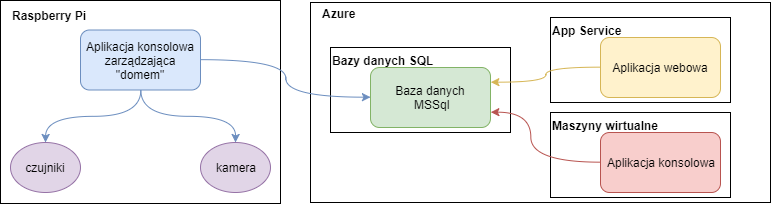
\includegraphics[scale=0.5]{budowa_azure.png}
	\caption{Podział systemu na usługi Azure}
	\label{fig:schemat_azure}
\end{figure}

\begin{figure}[H]
	\centering
	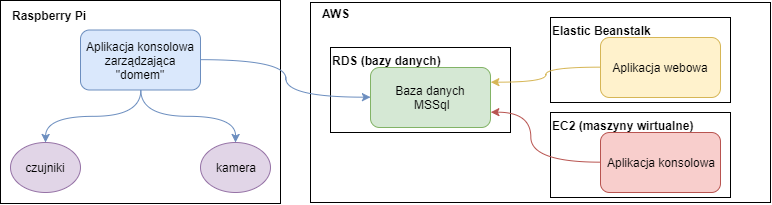
\includegraphics[scale=0.5]{budowa_aws.png}
	\caption{Podział systemu na usługi AWS}
	\label{fig:schemat_aws}
\end{figure}

